

\actTitle{Worksheet 4.7A}

\noindent \textbf{Instructions:}  Work together in groups of  3 or 4
to complete the following problems.

Student goals:
\begin{itemize}
\item Determine the restriction of the domain of a function in order
  to define an inverse.
\item State the canonical domain restrictions for sine, cosine, and
  tangent functions.
\item Use the definition of the arcsine, arccosine, and the arctangent
  functions to solve for one value in a trigonometric expression.
\item Sketch the graphs of the arcsine, arccosine, and the arctangent
  functions.
\item Compose trigonometric and inverse trigonometric functions to
  transform a trigonometric expression into an equivalent form that
  allows for direct algebraic manipulation to isolate a value in the
  domain of a trigonometric function in the original expression.
\item Determine equivalent expressions for the compositions of
  trigonometric and inverse trigonometric functions so that the
  results do not include any trigonometric functions.
\end{itemize}


\begin{enumerate}

\item Use the unit circle/reference triangles to determine the value of each of the following.
\begin{enumerate}
\item $\arcsin \left( \frac{\sqrt{2}}{2}\right)$
  \vfill
\item $\sin^{-1} \left( -\frac{\sqrt{3}}{2}\right)$
  \vfill
\item $\sin^{-1} \left( \frac{\sqrt{3}}{2}\right)$
  \vfill
\item $\arcsin \left( -\frac{1}{2}\right)$
  \vfill
\end{enumerate}


\item Use the unit circle/reference triangles to determine the value of each of the following.
\begin{enumerate}
\item $\arccos \left( \frac{\sqrt{2}}{2}\right)$
  \vfill
\item $\cos^{-1} \left( -\frac{\sqrt{3}}{2}\right)$
  \vfill
\item $\cos^{-1} \left( \frac{\sqrt{3}}{2}\right)$
  \vfill
\item $\arccos \left( -\frac{1}{2}\right)$
  \vfill
\end{enumerate}

\clearpage

\item Use the unit circle/reference triangles to determine the value of each of the following.
\begin{enumerate}
\item $\arctan \left( 1 \right)$
  \vfill
\item $\tan^{-1} \left( \frac{1}{\sqrt{3}}\right)$
  \vfill
\item $\tan^{-1} \left(\sqrt{3}\right)$
  \vfill
\item $\arctan \left( -1 \right)$
  \vfill
\end{enumerate}


\item Find the exact value of the expression.  Do not use a calculator.

\begin{enumerate}

\item $\arcsin \left(\sin\left(\frac{\pi}{3}\right)\right)=$
\vfill

\item $\arcsin \left(\sin\left(\frac{5\pi}{4}\right)\right)=$
\vfill

\item $\arccos \left(\cos\left(\frac{11\pi}{6}\right)\right)=$
\vfill


\item $\cos \left(\arccos\left( 0.56 \right)\right) = $
\vfill

\item $\tan \left( \arctan\left(1754\right) \right)=$
\vfill

\item $\arctan \left( \tan\left( \frac{23}{814}\right)\right)=$
\vfill

\end{enumerate}


\clearpage

\item Use a calculator to approximate the degree measure (to 1 decimal place) or radian measure (to 4 decimal places) of the angle $\theta$ subject to the given conditions. (\textbf{Hint:  }Use reference angles!)

\begin{enumerate}
\item $\displaystyle \cos(\theta)=-\frac{8}{11}$ and $180^\circ \leq \theta \leq 270^\circ$
\vfill
\item $\displaystyle \tan(\theta)=-\frac{9}{7}$ and $\frac{\pi}{2}<\theta< \pi$
\vfill
\item $\displaystyle \sin(\theta)=\frac{12}{19}$ and $90^\circ < \theta <180^\circ$
\vfill
\end{enumerate}


\clearpage



\item A student measures the length of the shadow of the Washington
  Monument to be 620 ft. If the Washington Monument is 555 ft tall,
  approximate the angle of elevation of the Sun to the nearest tenth
  of a degree.

  \vfill

\item A balloon advertising an open house is stabilized by two cables
  of lengths 20 ft and 40 ft tethered to the ground.  If the
  perpendicular distance from the balloon to the ground is
  $10\sqrt{3}$ ft, what is the degree measure of the angle each cable
  makes with the ground?  Round to the nearest tenth of a
  \textbf{degree} if necessary.

  \vfill


\end{enumerate}


\hwTitle{Section 4.7A}

\begin{enumerate}
\item Determine the radian measure of $\phi$ associated with the
  coordinate in the figure below. (Numerical answers should be to
  within 2 decimal digits.)
      
  \begin{tikzpicture}[y=1.0cm, x=1.0cm,font=\sffamily]
    \draw[thick,black] (-2,0) -- (2,0) node[anchor=west] {$x$};
    \draw[thick,black] (0,-2) -- (0,2) node[anchor=south] {$y$};
    \draw[thin,black] (0,0) -- (-1,-1.8);
    \draw[thin,black] (0.3,0) arc (0:240:0.3);
    \node[black,xshift=-15.4,yshift=-8.2] at (0,0) {$\phi$};
    \node[black,anchor=north east] at (-1,-1.8) {$(-2,-2\sqrt{3})$};
    \draw[black,fill=black] (-1,-1.8) circle (0.5ex);
  \end{tikzpicture}
  
\item Determine the radian measure of $\alpha$ where $\alpha$ is
  between $\frac{\pi}{2}$ and $\pi$ and $\sin(\alpha)=\frac{1}{2}$.
  (Numerical answers should be to within 2 decimal digits.)

\item Determine the radian measure of $\beta$ in the figure below.
    
  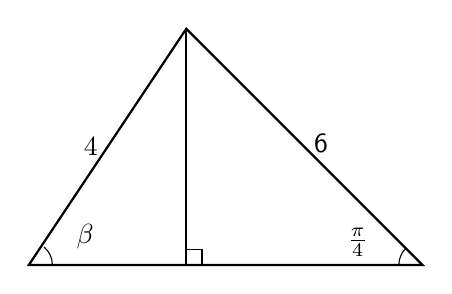
\begin{tikzpicture}[y=1.0cm, x=1.0cm,font=\sffamily]
    \draw[thick,black] (0,0) -- (2,3) -- (5,0) -- cycle;
    \draw[thick,black] (2,3) -- (2,0);
    \draw[thin,black] (2,0.2) -- (2.2,0.2) -- (2.2,0); 
    \draw[thin,black] (4.7,0) arc (180:135:0.3);
    \draw[thin,black] (0.3,0) arc (0:50:0.3);
    \node[black,xshift=-23.4,yshift=8.2] at (5,0) {$\frac{\pi}{4}$};
    \node[black,xshift=20.4,yshift=10.2] at (0,0) {$\beta$};
    \node[black,anchor=south west] at (3.5,1.3) {6};
    \node[black,anchor=east] at (1,1.5) {$4$};
  \end{tikzpicture}

\item The area of the shaded region on the unit circle shown in the
  figure below is 0.9. Determine the radian measure of the angle
  $\gamma$.

  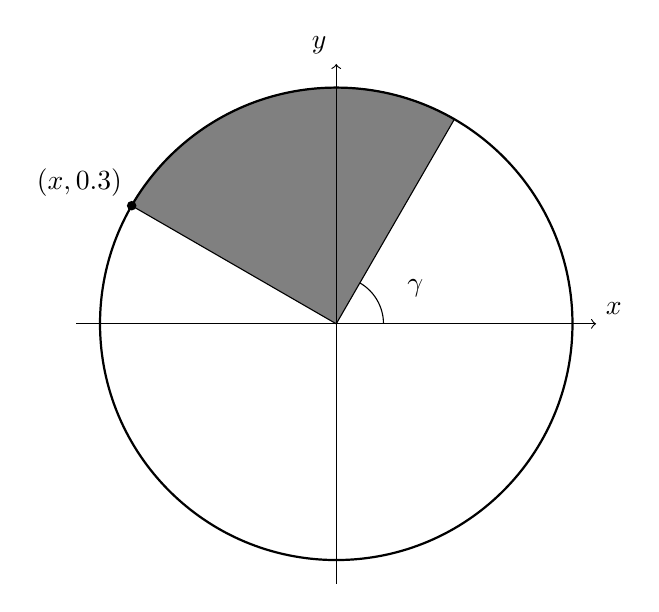
\begin{tikzpicture}[y=1.5cm, x=1.5cm,font=\sffamily]
    \draw[thin,black,fill=gray] (0,0) -- (60:2) arc (60:150:2) -- (0,0);
    \fill[black] (150:2) circle [radius=0.4ex] node[anchor=south east] {$(x,0.3)$};
    % \shade[gray] (0,0) -- (60:2) arc (60:150:2) -- (0,0);
    \draw[thick,black] (0,0) circle (2);
    \draw[thin,black] (0.4,0) arc (0:60:0.4);
    %\draw[thin,black] (150:0.4) arc (150:180:0.4);
    \draw[thin,black,->] (-2.2,0.0) -- (2.2,0.0) node[anchor=south west] {$x$};
    \draw[thin,black,->] (0.0,-2.2) -- (0.0,2.2) node[anchor=south east] {$y$};
    \node[black,anchor=west] at (30:0.6) {$\gamma$};
  \end{tikzpicture}


\end{enumerate}
